\documentclass{beamer}
\usetheme{Pittsburgh}
\beamertemplatenavigationsymbolsempty


\usepackage{amsmath}
\usepackage{amssymb}
\usepackage{bm} % For bold math symbols
\usepackage{graphicx}
\usepackage{tikz}



\usepackage{subfig} % Changed from subfigure (deprecated)
\usepackage{multirow}
\usepackage{multicol}
\usepackage{color}
\usepackage{url}
\usepackage{hyperref}
\usepackage{listings}
\usepackage[noend]{algorithm}
\usepackage{physics} 

\usepackage{animate}

% add image path
\graphicspath{{Images/}}






\DeclareMathOperator{\argmin}{argmin}
\DeclareMathOperator{\argmax}{argmax}






\title{Weekly Updates\\
\tiny{Wednesday, 03/04/2025}}
\author{Andrea Bonifacio}
\date{}

\begin{document}

\begin{frame}
\titlepage
\end{frame}


\begin{frame}{Two Main Challenges}
    \begin{columns}
        \begin{column}{0.48\textwidth}
            \textbf{Issue 1: Energy Minimization in Training}
            \begin{itemize}
                \item Current network achieves some energy minimization
                \item But reduction is a small fraction of the total energy
                \item Based on my observations, origin constraint seems to affect energy minimization, either a correct rest position prediction or some true non-linear modes. 
            \end{itemize}
        \end{column}
        
        \begin{column}{0.48\textwidth}
            \textbf{Issue 2: Correct Objective Function}
            \begin{itemize}
                \item They propose an objective function based on the energy minimization
                \item But in one of their simulations additional terms are needed
            \end{itemize}
        \end{column}
    \end{columns}
\end{frame}


\begin{frame}
    \frametitle{Example of the issue}
    \begin{itemize}
        \item The network has learned to minimize the internal energy, but has no control on the linear modes output, which dominates the simulation.
        \item Objective function used:
        \[
              z_{n+1} = \underset{z}{\argmin}  \frac{1}{2h^2} \norm{n(z) - 2u_n + u_{n-1}}^2_M + E(n(z))
        \]
    \end{itemize}
\end{frame}

\begin{frame}
    \frametitle{Animation}
    \begin{center}
        \animategraphics[width=0.8\textwidth, autoplay, loop]{12}{Images/beam_linear/frames/frame}{0}{27}
    \end{center}
\end{frame}

\begin{frame}
    \frametitle{ Corrected Energy Calculation}
    This plot shows the energy calculation for the validation using a twisted beam. The energy from the FEM simulation and the neural network are in a similar range until the prediction of the network diverges, then the energy shoots up. The formula has been corrected, but there are still minimal differences when the displacements are similar. 
    \begin{center}
        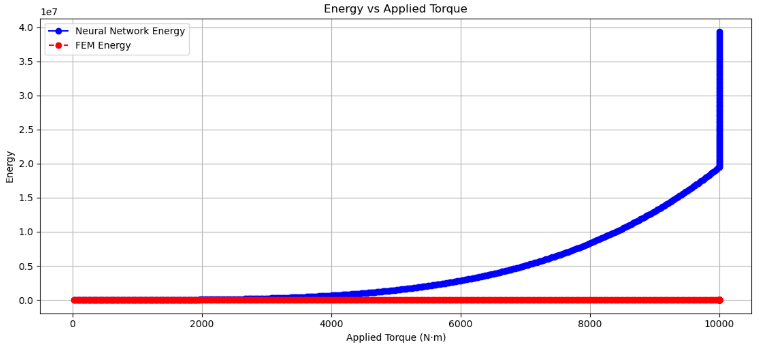
\includegraphics[width=0.8\textwidth]{Images/fem_vs_nn_energy.png}
    \end{center}
   
\end{frame}

% \begin{frame}
%     \frametitle{Network Architecture}
%     \begin{itemize}
%         \item The network is a feedforward neural network.
%         \item The input is the modal coordinate \( z \in \mathbb{R}^m \).
%         \item The output is a correction on the displacement field \( \mathbf{y} \in \mathbb{R}^n \).
%     \end{itemize}
%     \begin{center}
            
%             \begin{tikzpicture}
%                 % Modal coordinate (z)
%                 \draw[fill=green!20] (-3, 1) rectangle (-2.5,2);
%                 \node at (-2.75, 1.5) {$z$}; % Label inside the rectangle
                
%                 % Displacement (u)
%                 \draw[fill=green!20] (2.5,0) rectangle (3,3);
%                 \node at (2.75, 1.5) {$y$}; % Label inside the rectangle
                
%                 % Energy loss transition
%                 \draw[fill=blue!60,opacity=0.8] (-2,1) -- (2,-0) -- (2,3) -- (-2,2) -- cycle;
%                 \node[below] at (0,-1) {\textbf{Energy loss}};
                
%                 % Energy loss arrow
%                 \draw[thick,blue,->] (-2,-0.8) -- (2,-0.8);
%             \end{tikzpicture}
%     \end{center}
% \end{frame}




\begin{frame}
    \frametitle{Challenges \& Next Steps}
        \begin{itemize}
            \item I am open to suggestions on how to proceed, I don't really have an idea.
            \item In the paper they mention that without the origin constraint, the network wrongly predicts the rest position, but in my experience that is limiting the energy minimization.
        \end{itemize}
\end{frame}

% Q&A
\begin{frame}
    \begin{center}
        \color{blue} \Huge{Questions?}
    \end{center}

\end{frame}
\end{document}

